\documentclass[11pt,a4paper]{article}

\usepackage[margin=2.4cm]{geometry}
\usepackage{amsmath,amssymb,bm,booktabs,tabularx}
\usepackage{graphicx}
\usepackage{microtype}
\usepackage{float}
\usepackage{caption}
\usepackage{enumitem}
\usepackage{hyperref}
\usepackage{xurl}

\hypersetup{
    colorlinks=true,
    linkcolor=blue,
    citecolor=blue,
    urlcolor=blue
}

\graphicspath{{figures/}}
\setlength{\parskip}{0.35em}
\setlength{\parindent}{2em}

\title{Geometric Structure of GO Label Probes in Protein-Language-Model
Embeddings:\\
Spectral Concentration Is Explained by Label Co-Occurrence}

\author{
    Ruixi Ma\\
    Rutgers University
    \\[1.0em]
    \normalsize with contributions from Guillaume Lamoureux\\
    \normalsize Rutgers University
}

\date{October 2026}

\begin{document}

\maketitle

\begin{abstract}
Linear probes trained on protein-language-model embeddings are often read as
revealing the directions along which a biological property is encoded. We test how
far that reading is supported for 75 Gene Ontology Cellular Component (GO CC)
labels represented in 480-dimensional ESM-2 embeddings of 9{,}895 proteins.

The stacked probe weight matrix $W \in \mathbb{R}^{75 \times 480}$ is linearly
independent (numerical rank 75) and has no near-collinear pair: the largest
absolute cosine similarity between any two label directions is $0.4177$, an angle
of about $65^\circ$. Its singular-value spectrum is moderately concentrated: 90\%
of the squared spectral energy lies in 49 of the 75 directions, and the effective
rank is 54.54.

We then ask whether that concentration is a property of the sequence
representation. Three null models are compared, each preserving a different part of
the problem. Random directions with matched row norms are less concentrated than
the observed matrix (effective rank 60.91, $p < 0.001$), and weights fitted to
column-shuffled labels are also less concentrated once row norms are matched (57.75,
$p = 0.005$). However, a row-permutation null that preserves the co-occurrence
structure of the labels but breaks its association with the proteins reproduces the
observed spectrum almost exactly (54.32, $p = 0.73$).

The concentration is therefore inherited from the statistical structure of the GO
labels rather than from protein-specific information extracted by the probe. This
is also what the geometry of the problem predicts: with 75 labels in 480
dimensions there is no capacity pressure that would call for superposition in the
first place. Pairwise weight similarity still tracks label co-annotation after
controlling for co-occurrence (partial rank correlation 0.4889), so the geometry
carries semantic information, but it is not independent evidence of feature
superposition.
\end{abstract}

\section{Introduction}

Pretrained protein language models map amino-acid sequences to continuous vectors.
If such a vector contains information about subcellular localization, a linear
classifier can recover part of it, and its weight vector is often interpreted as
the direction along which the model represents the corresponding property.

This interpretation becomes more interesting when several labels appear to share
directions. Elhage et al.\ \cite{elhage2022toy} describe \emph{superposition}: a
network may encode more features than it has dimensions, allowing features to share
directions at the cost of interference. A natural question is whether the weight
vectors of many GO labels, trained independently on the same embeddings, display a
similar phenomenon.

That analogy needs care. A probe is a supervised read-out fitted on frozen
features, not a description of the model's internal computation, and a shared
direction between two probes can arise for entirely mundane reasons: the labels are
correlated, the embedding covariance is anisotropic, or the training procedure
regularizes in a particular way. Evidence for superposition therefore has to
distinguish geometric structure that follows from the label distribution from
structure that the representation itself contributes.

This report asks four questions about the weight matrix $W$ of 75 GO CC probes:

\begin{enumerate}[label=\textbf{Q\arabic*.},leftmargin=*]
    \item Are any two weight vectors exactly collinear?
    \item Do any three weight vectors span a subspace of dimension less than three?
    \item Is any subset of $M$ weight vectors rank-deficient?
    \item Even without exact dependence, is the spectrum of $W$ concentrated beyond
    what a suitable null model produces?
\end{enumerate}

Questions Q1--Q3 have clean linear-algebraic answers. Q4 is the substantive one,
because approximate shared structure is what machine-learning models actually
exhibit at finite numerical precision, and because a positive answer only becomes
meaningful once the null model is specified.

Our contribution is threefold. First, we answer Q1--Q3 with quantitative margins
rather than a rank test alone. Second, we quantify the spectral concentration and
show that it is moderate, not a collapse onto a few directions. Third, and most
importantly, we compare the observed spectrum against a ladder of null models that
preserve progressively more of the label structure, and show that the
concentration is reproduced when the labels' co-occurrence pattern is preserved but
their association with the proteins is broken.

That last result changes the interpretation a concentrated spectrum would
otherwise invite. The concentration is real, but it is a property of the GO label
distribution as seen through a linear read-out, not evidence that ESM-2 spreads
biological features across shared directions.

\section{Data and Model}

\subsection{Dataset}

We download reviewed (Swiss-Prot) entries from the UniProtKB REST API and keep
those with at least one GO Cellular Component annotation
\cite{uniprotEmbeddings,geneontology2021}. The
download is capped at 10{,}000 records, which keeps the experiment reproducible on a
laptop; the resulting dataset is a prefix of reviewed Swiss-Prot rather than the
full database. Entries without an accession, sequence, or GO CC annotation are
dropped, and the 75 GO CC terms carried by at least 100 proteins are kept. Every
sequence is embedded with ESM-2 \texttt{esm2\_t12\_35M\_UR50D} \cite{lin2023esm},
using the mean of the layer-12 states over the residues (excluding the BOS and EOS
tokens) as the protein vector. Table~\ref{tab:data} summarises the dataset.

\begin{table}[H]
\centering
\caption{Dataset used in this study.}
\label{tab:data}
\begin{tabular}{lr}
\toprule
Item & Value \\
\midrule
Protein records & 9{,}895 \\
Embedding dimension & 480 \\
Selected GO CC labels & 75 \\
Distinct GO CC terms in the export & 1{,}779 \\
Label matrix $Y$ & $9895 \times 75$ \\
Positive label assignments & 36{,}188 \\
Mean labels per protein & 3.6572 \\
Proteins with at least one selected label & 9{,}786 \\
Embedding matrix $X$ & $9895 \times 480$ \\
\bottomrule
\end{tabular}
\end{table}

\subsection{Linear probe}

For protein $n$ with embedding $x_n \in \mathbb{R}^{480}$ and label vector
$y_n \in \{0,1\}^{75}$, a one-vs-rest logistic regression is fitted with balanced
class weights and $L_2$ regularization $C = 1$:

\begin{equation}
p(y_{ni}=1 \mid x_n) = \sigma(w_i^\top x_n + b_i),
\qquad
\sigma(z) = \frac{1}{1+e^{-z}}.
\end{equation}

Stacking the 75 coefficient vectors gives

\begin{equation}
W =
\begin{bmatrix}
w_1^\top \\ \vdots \\ w_{75}^\top
\end{bmatrix}
\in \mathbb{R}^{75 \times 480},
\end{equation}

whose rows are the objects of study. The embeddings are standardised inside the
pipeline, so $W$ is expressed in the standardized coordinate system.

A single 80/20 split with a fixed seed (42) gives 7{,}916 training and 1{,}979 test
proteins. On the test split the mean ROC-AUC is 0.7841 and the mean average
precision is 0.2226, averaged over the labels that contain both classes in the
fold. The probe is therefore informative, but the performance metrics say nothing
about the geometry analysed below; they are reported to establish that $W$ is a
meaningful read-out rather than an artefact of an untrained model.

\section{Methods}

\subsection{Exact linear dependence (Q1--Q3)}

For two nonzero weight vectors, the cosine similarity is

\begin{equation}
c_{ij} = \frac{w_i^\top w_j}{\lVert w_i \rVert_2 \, \lVert w_j \rVert_2}.
\end{equation}

The vectors are collinear exactly when $|c_{ij}| = 1$, equivalently when
$\operatorname{rank}([w_i^\top; w_j^\top]) < 2$. The absolute value is needed
because antiparallel vectors are also linearly dependent.

A rank test alone says little about how far a matrix is from dependence. For two
unit vectors with cosine $c$, the singular values of the $2 \times 480$ stack are
$\sigma_1^2 = 2(1+|c|)$ and $\sigma_2^2 = 2(1-|c|)$, so

\begin{equation}
\frac{\sigma_2}{\sigma_1} = \sqrt{\frac{1-|c|}{1+|c|}}.
\end{equation}

This ratio turns a cosine into a collinearity margin and is reported together with
the rank. Numerical ranks use the standard tolerance
$\max(m,n)\,\epsilon\,\sigma_1$ with $\epsilon$ the machine epsilon.

Q2 and Q3 are logical consequences of Q1 for a full-row-rank matrix: any subset of
linearly independent rows is also independent. We nevertheless verify them
numerically on random row subsets, which also serves as a check on the tolerance.

\subsection{Spectral concentration (Q4)}

The singular value decomposition of $W$ is

\begin{equation}
W = U \Sigma V^\top, \qquad \sigma_1 \geq \cdots \geq \sigma_{75} \geq 0 .
\end{equation}

The squared singular values measure the energy along each orthogonal direction. We
report the cumulative energy

\begin{equation}
E(k) = \frac{\sum_{i=1}^{k}\sigma_i^2}{\sum_{i=1}^{75}\sigma_i^2},
\end{equation}

the number of directions needed for 90\% and 95\% of the energy (Rank90, Rank95),
and the effective rank

\begin{equation}
r_{\mathrm{eff}} = \exp\left(-\sum_{i:\,p_i>0} p_i \log p_i\right),
\qquad p_i = \frac{\sigma_i^2}{\sum_j \sigma_j^2}.
\end{equation}

Effective rank is the continuous analogue of algebraic rank: it equals 75 for a
flat spectrum and approaches 1 for a rank-one matrix.

\subsection{Null models}
\label{sec:nulls}

A concentration statistic is only interpretable relative to a null. We use three,
chosen so that each preserves a different part of the original problem
(Table~\ref{tab:nulls}).

\begin{table}[H]
\centering
\caption{Null models. Each row states what is randomized and what is held fixed.}
\label{tab:nulls}
\begin{tabularx}{\textwidth}{@{}lXX@{}}
\toprule
Null & Randomized & Preserved \\
\midrule
Isotropic directions & the direction of every row, redrawn from a Gaussian &
row norms, matrix shape \\
Label shuffle & each label column, independently & number of positives per label,
training embeddings \\
Row permutation & the pairing between proteins and label vectors, by permuting the
rows of $Y$ as a block & label co-occurrence structure, label prevalence,
training embeddings \\
\bottomrule
\end{tabularx}
\end{table}

In every case the random weight matrix is rescaled so that its row norms match
those of the observed $W$. Row norms matter because the spectrum of a matrix
depends on its magnitude profile as well as on the angles between rows; without
matching, a null can land on either side of the observation for reasons unrelated
to direction structure. The label-shuffle null is therefore evaluated both raw and
matched, and the contrast between the two is itself informative.

For a statistic $T$ where lower values mean more concentration, the empirical
lower-tail $p$-value over $B$ draws is

\begin{equation}
p = \frac{1 + \#\{T_b \leq T_{\text{obs}}\}}{1 + B}.
\end{equation}

All nulls use fixed seeds (42 for the isotropic and label-shuffle nulls, 2026 for
the row-permutation null) and are computed on the same training embeddings and the
same probe hyper-parameters as the observed matrix.

\subsection{Association with label structure}

If the geometry follows the labels, labels that are annotated together should
receive similar probe directions. For each of the $\binom{75}{2} = 2{,}775$
unordered label pairs we compute the label correlation $r_{ij}$ (Pearson
correlation of the two binary columns), the co-occurrence count $q_{ij}$, and the
weight cosine $c_{ij}$.

The monotone association between $c_{ij}$ and $r_{ij}$ is measured with Spearman's
rank correlation. Because both quantities grow with label frequency, we also
compute a residualized version: $c_{ij}$ and $r_{ij}$ are rank-transformed, each is
regressed on an intercept and the rank of $\log(1+q_{ij})$, and the correlation of
the residuals is reported. This controls for co-occurrence rank only; it does not
control for ontology structure or label prevalence.

\section{Results}

\subsection{Exact geometry: no dependence, with a wide margin}

The weight matrix has shape $75 \times 480$ and numerical rank 75 (tolerance
$4.5 \times 10^{-12}$). Every random subset of rows is full rank, including
samples of all 75 rows (Table~\ref{tab:subsets}).

\begin{table}[H]
\centering
\caption{Rank of random row subsets (100 samples per subset size).}
\label{tab:subsets}
\begin{tabular}{rrr}
\toprule
$M$ & Mean rank & Rank-deficient subsets \\
\midrule
2  & 2.00  & 0/100 \\
3  & 3.00  & 0/100 \\
5  & 5.00  & 0/100 \\
10 & 10.00 & 0/100 \\
20 & 20.00 & 0/100 \\
40 & 40.00 & 0/100 \\
75 & 75.00 & 0/100 \\
\bottomrule
\end{tabular}
\end{table}

The margins are wide. The most similar pair of weight vectors is
\texttt{GO:0005789} (endoplasmic reticulum membrane) and \texttt{GO:0005783}
(endoplasmic reticulum), with $|c| = 0.4177$; the corresponding angle is
$65.3^\circ$ and $\sigma_2/\sigma_1 = 0.641$. The most anti-aligned pair reaches
$c = -0.161$, and the mean absolute cosine over all pairs is $0.063$. No triple or
larger subset is degenerate.

The negative answer to Q1--Q3 is therefore robust to the choice of tolerance: it is
not a borderline numerical call.

\subsection{Spectral concentration}

The spectrum decays gradually (Figure~\ref{fig:sv}). The leading singular value is
$\sigma_1 = 41.96$ and accounts for 7.6\% of the total energy; the first 20
directions account for 54.7\%. The 90\% level is reached at $k = 49$ and the 95\%
level at $k = 57$ (Figure~\ref{fig:energy}, Table~\ref{tab:spectrum}). The effective
rank is 54.54 out of a possible 75.

\begin{table}[H]
\centering
\caption{Spectral summary of $W$.}
\label{tab:spectrum}
\begin{tabular}{lr}
\toprule
Quantity & Value \\
\midrule
$\sigma_1$ & 41.96 \\
Rank90 & 49 \\
Rank95 & 57 \\
Effective rank & 54.54 \\
Maximum attainable rank & 75 \\
Mean absolute cosine between rows & 0.063 \\
\bottomrule
\end{tabular}
\end{table}

\begin{figure}[H]
\centering
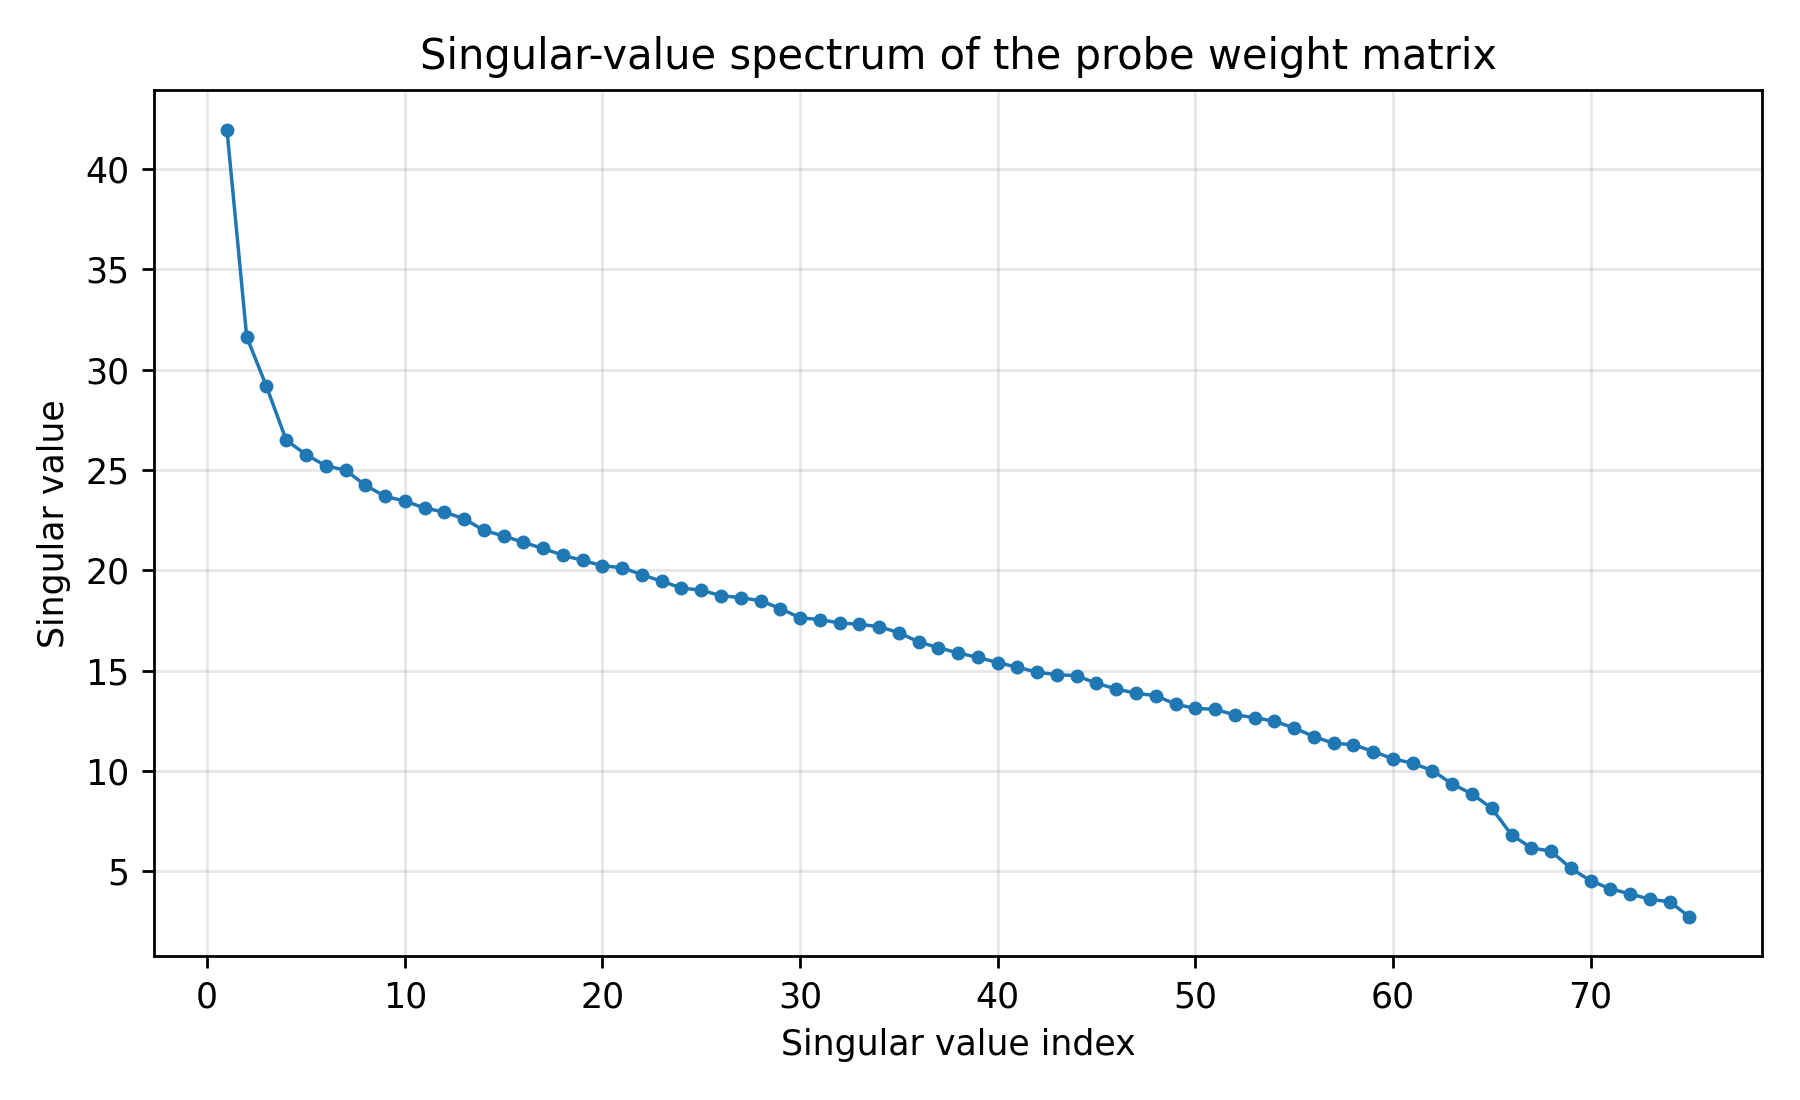
\includegraphics[width=0.80\textwidth]{fig_singular_values.png}
\caption{Singular-value spectrum of the probe weight matrix. The decay is
continuous: there is no gap separating a small leading subspace from the rest.}
\label{fig:sv}
\end{figure}

\begin{figure}[H]
\centering
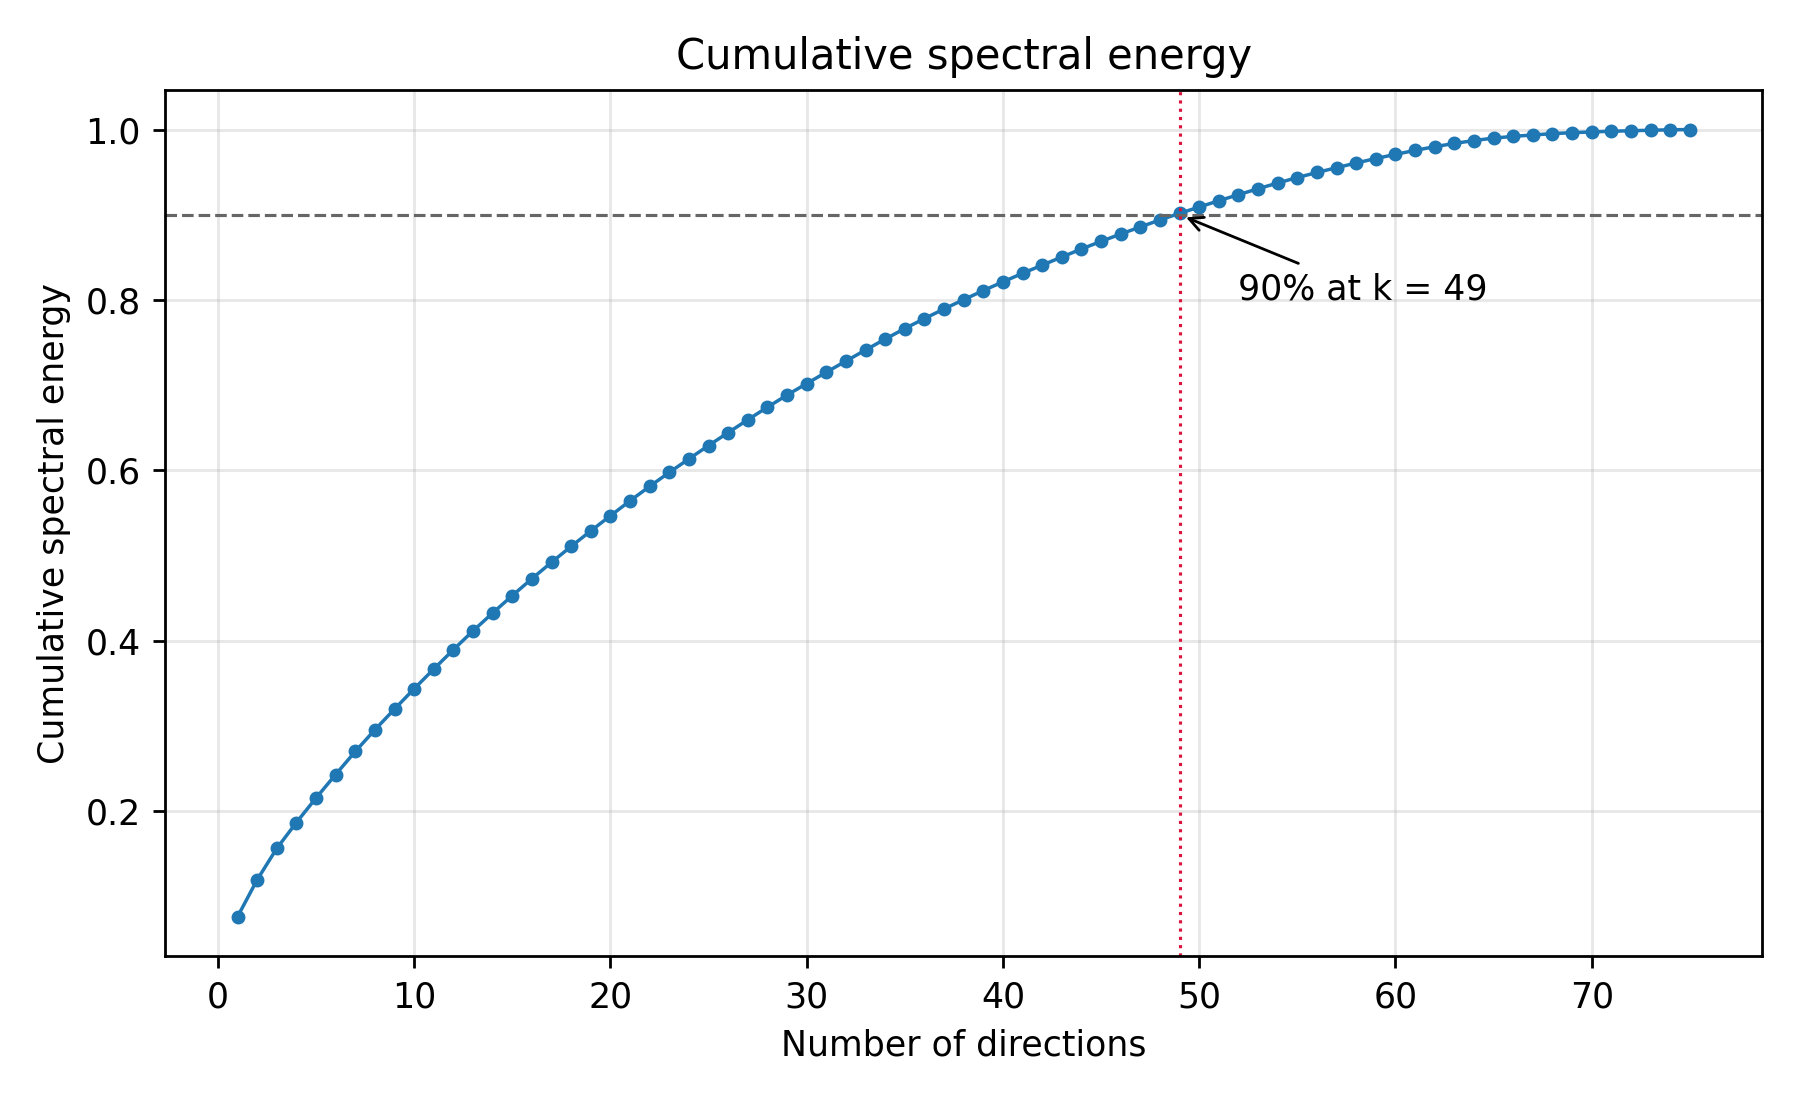
\includegraphics[width=0.80\textwidth]{fig_cumulative_energy.png}
\caption{Cumulative spectral energy. The dotted line marks the 90\% level, reached
at 49 of the 75 directions.}
\label{fig:energy}
\end{figure}

The concentration is moderate. A matrix that genuinely occupied a 5- or
10-dimensional subspace would reach 90\% of its energy within a handful of
directions and show a sharp spectral gap; here the curve is close to linear through
the middle of the spectrum, and two thirds of the directions are still needed to
reach 90\%.

\subsection{The concentration is reproduced by label structure alone}

Figure~\ref{fig:ladder} and Table~\ref{tab:ladder} compare the observed spectrum
with the null models of Section~\ref{sec:nulls}.

\begin{table}[H]
\centering
\caption{Null models compared with the observed spectrum. Intervals are 95\%
empirical intervals; $p$-values are lower-tail. Lower values mean more
concentration.}
\label{tab:ladder}
\begin{tabular}{lccccc}
\toprule
Null & $B$ & Effective rank & $p$ & Rank90 & $p$ \\
\midrule
Observed $W$ & -- & 54.54 & -- & 49 & -- \\
Isotropic directions & 1000 & 60.91 [60.66, 61.14] & $<0.001$ & 51.96 [51, 52] & $<0.001$ \\
Label shuffle, raw & 200 & 52.51 [52.04, 53.03] & 1.000 & 44.24 [44, 45] & 1.000 \\
Label shuffle, matched & 200 & 57.75 [57.36, 58.16] & 0.005 & 49.65 [49, 50] & 0.358 \\
Row permutation & 100 & 54.32 [53.57, 54.98] & 0.733 & 47.98 [48, 48] & 1.000 \\
\bottomrule
\end{tabular}
\end{table}

\begin{figure}[H]
\centering
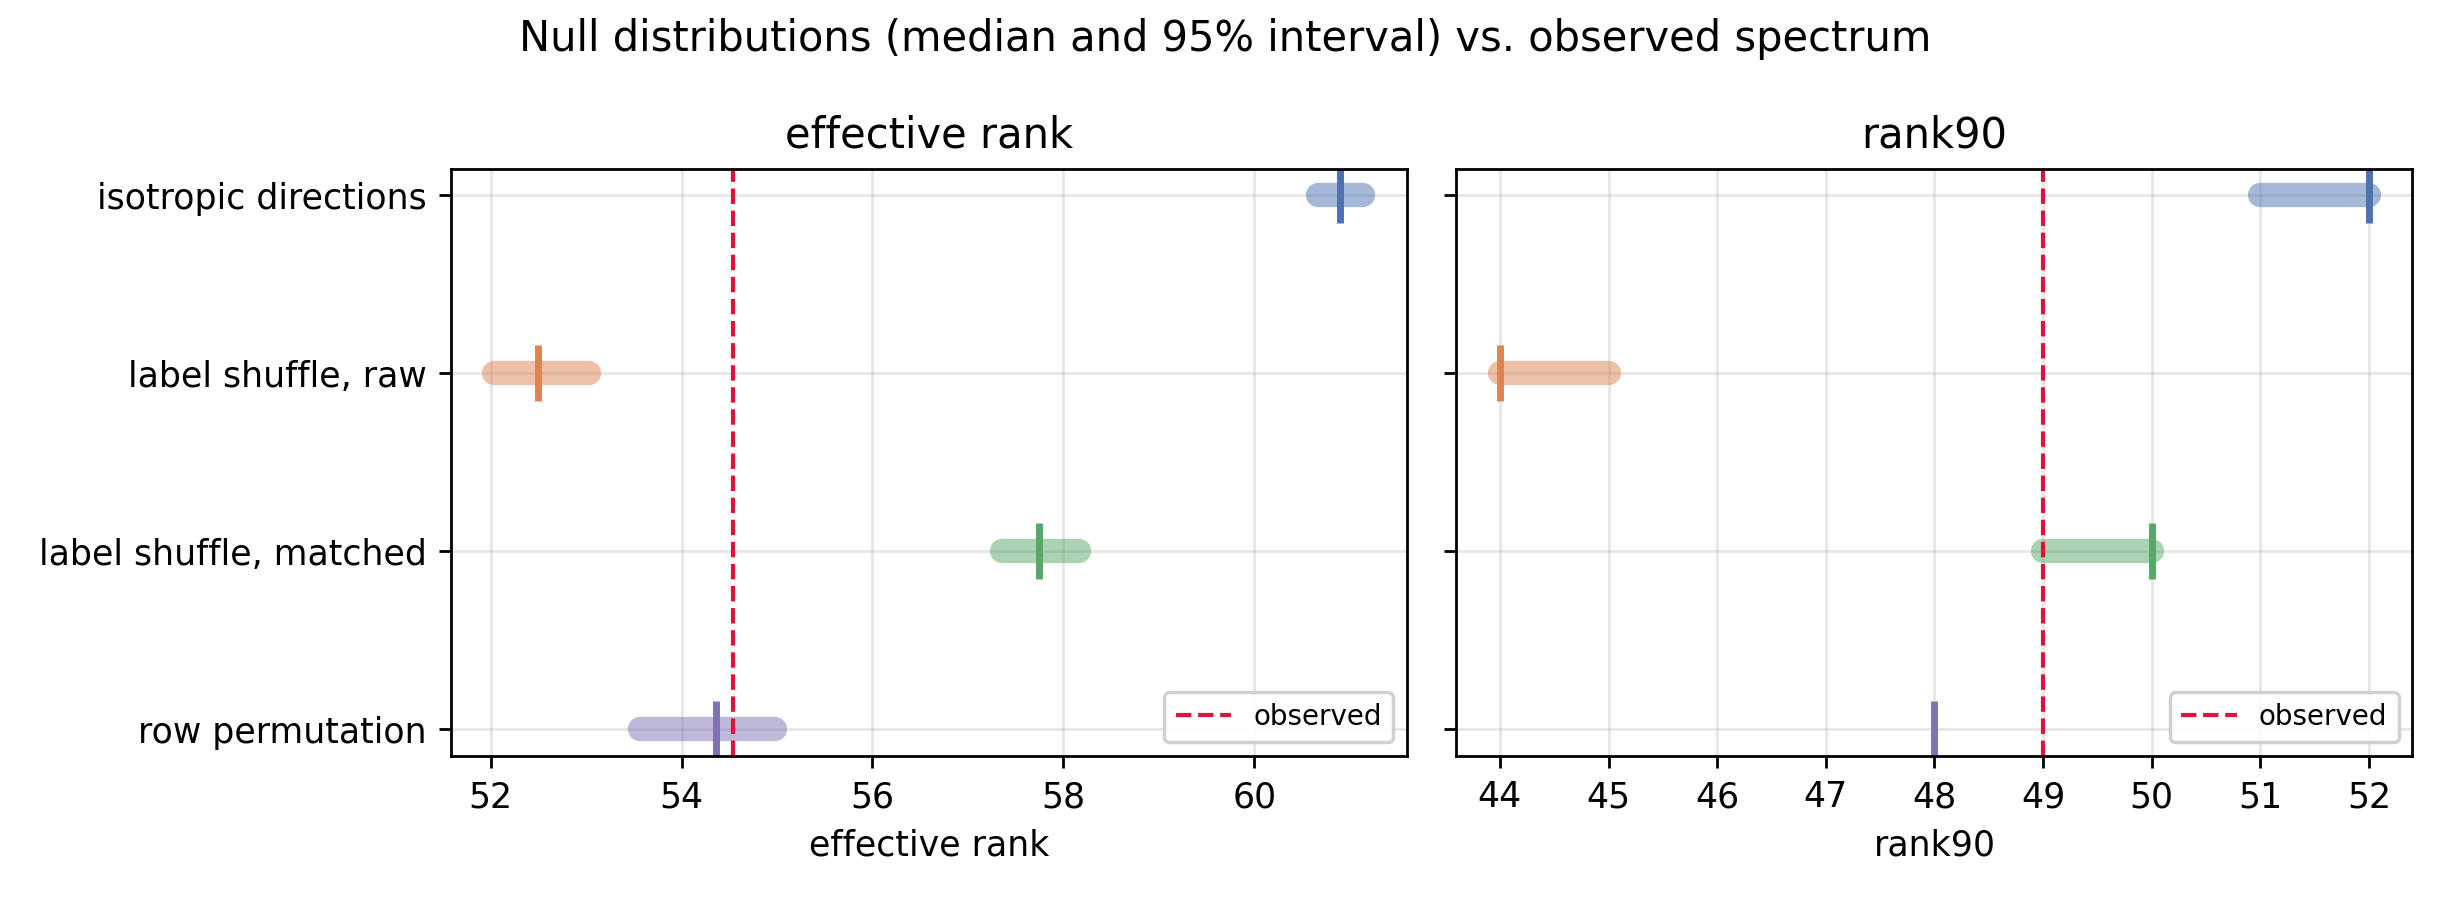
\includegraphics[width=\textwidth]{fig_null_ladder.png}
\caption{Null distributions (median and 95\% interval) against the observed
effective rank and Rank90. The row-permutation null is the only one that coincides
with the observation.}
\label{fig:ladder}
\end{figure}

Read from top to bottom, the table is a ladder. Random directions of the right
magnitude are less concentrated than $W$ ($p < 0.001$), so the weights are not
noise. Shuffling labels destroys the co-occurrence pattern and moves the null
further from the observation. Keeping the co-occurrence pattern while breaking its
association with the proteins brings the null to 54.32, against an observed 54.54
($p = 0.73$) and a Rank90 of 47.98 against 49.

The last row is decisive for the interpretation. If the observed spectrum is what
one obtains by fitting the same probe to label vectors that carry the correct
co-occurrence structure but are attached to the wrong proteins, then the spectrum
is a consequence of the label distribution and the regression, not of
protein-specific information in the embeddings. The sequence representation still
carries predictive signal (mean ROC-AUC 0.784), but the concentration of $W$ is not
evidence of additional geometric structure contributed by that representation.

The raw label-shuffle row is a reminder that null definitions matter: without
matching row norms it is \emph{more} concentrated than the observation ($p = 1.0$
in the lower tail). A study that quoted only that row would reach the opposite
conclusion. Every null in this report is therefore reported with its matching rule
and its direction of comparison.

\subsection{Weight similarity tracks label co-annotation}

Figure~\ref{fig:scatter} shows the association between label correlation and
weight-vector cosine over all 2,775 pairs, and Figure~\ref{fig:cosine} shows the
full cosine matrix.

\begin{figure}[H]
\centering
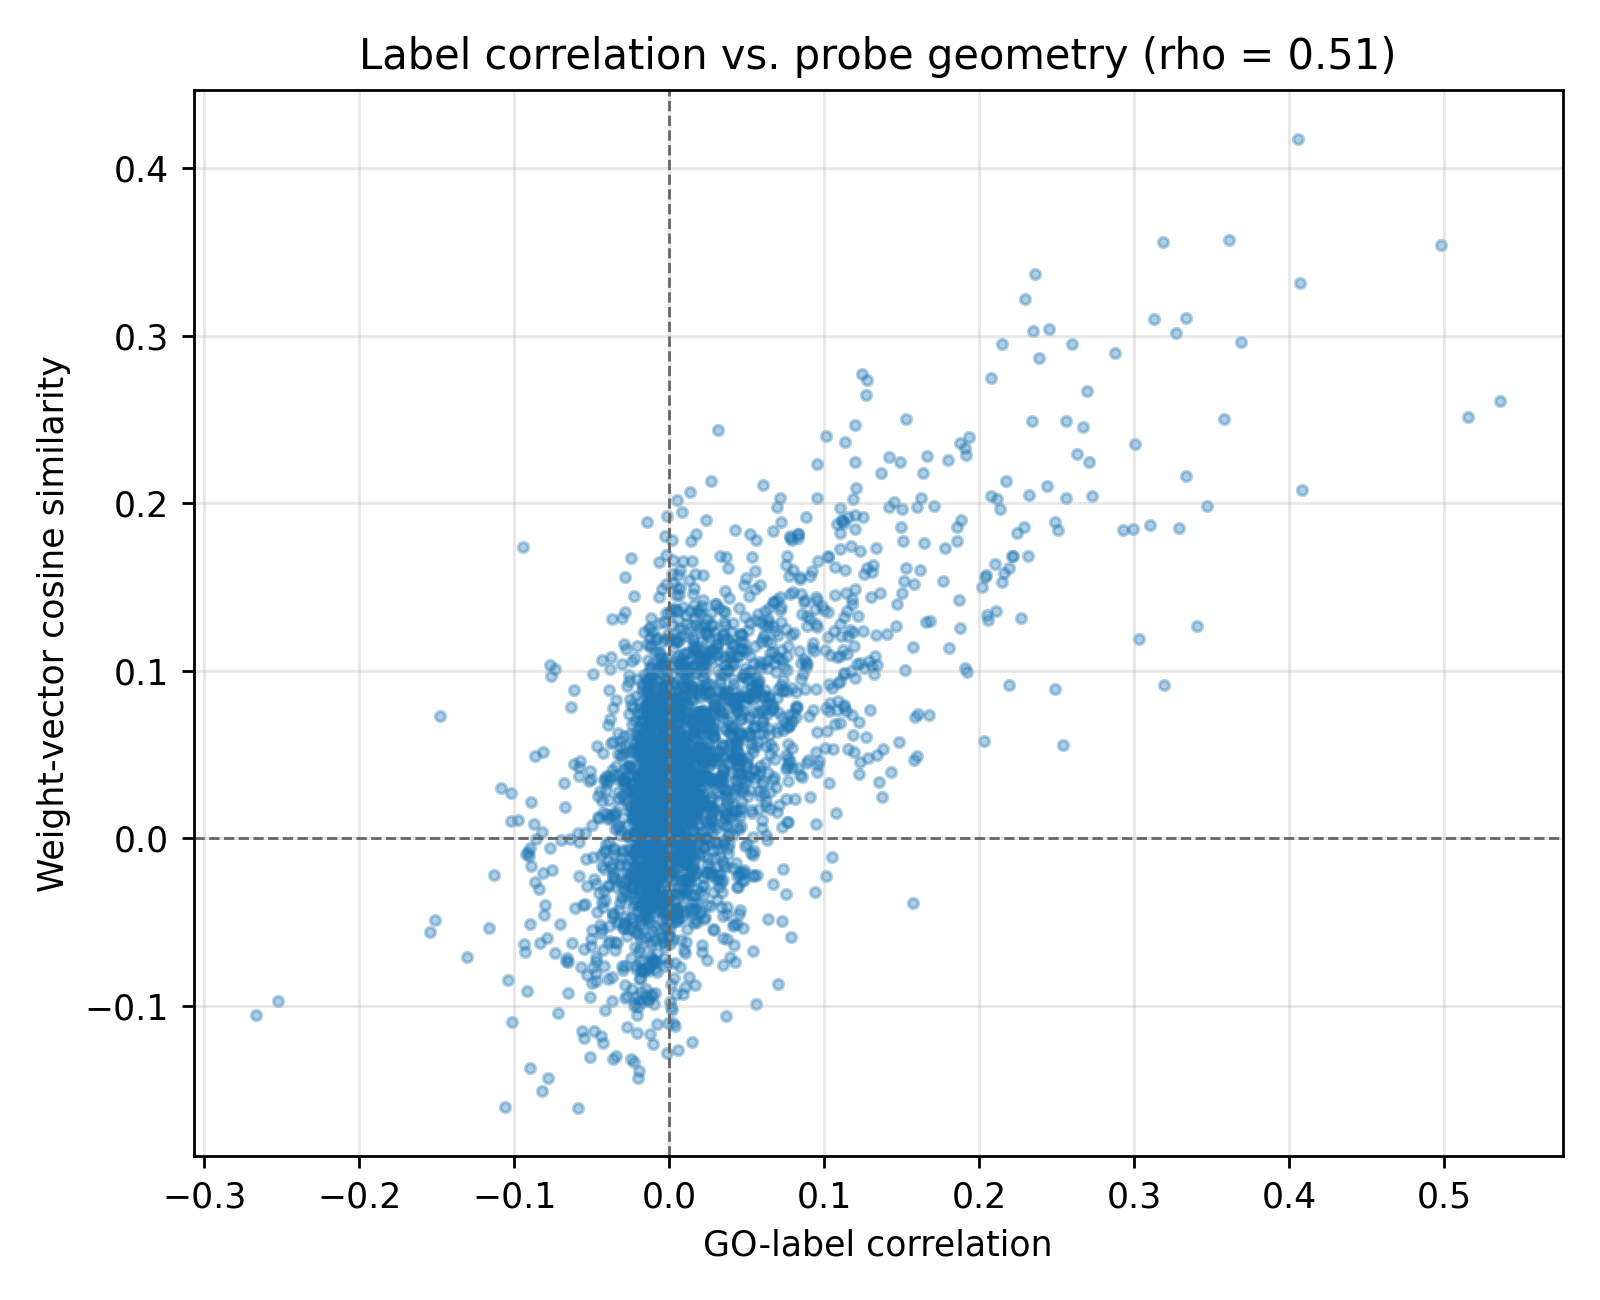
\includegraphics[width=0.78\textwidth]{fig_weight_vs_label_correlation.png}
\caption{Label correlation against probe weight-vector cosine similarity, one point
per unordered label pair.}
\label{fig:scatter}
\end{figure}

\begin{figure}[H]
\centering
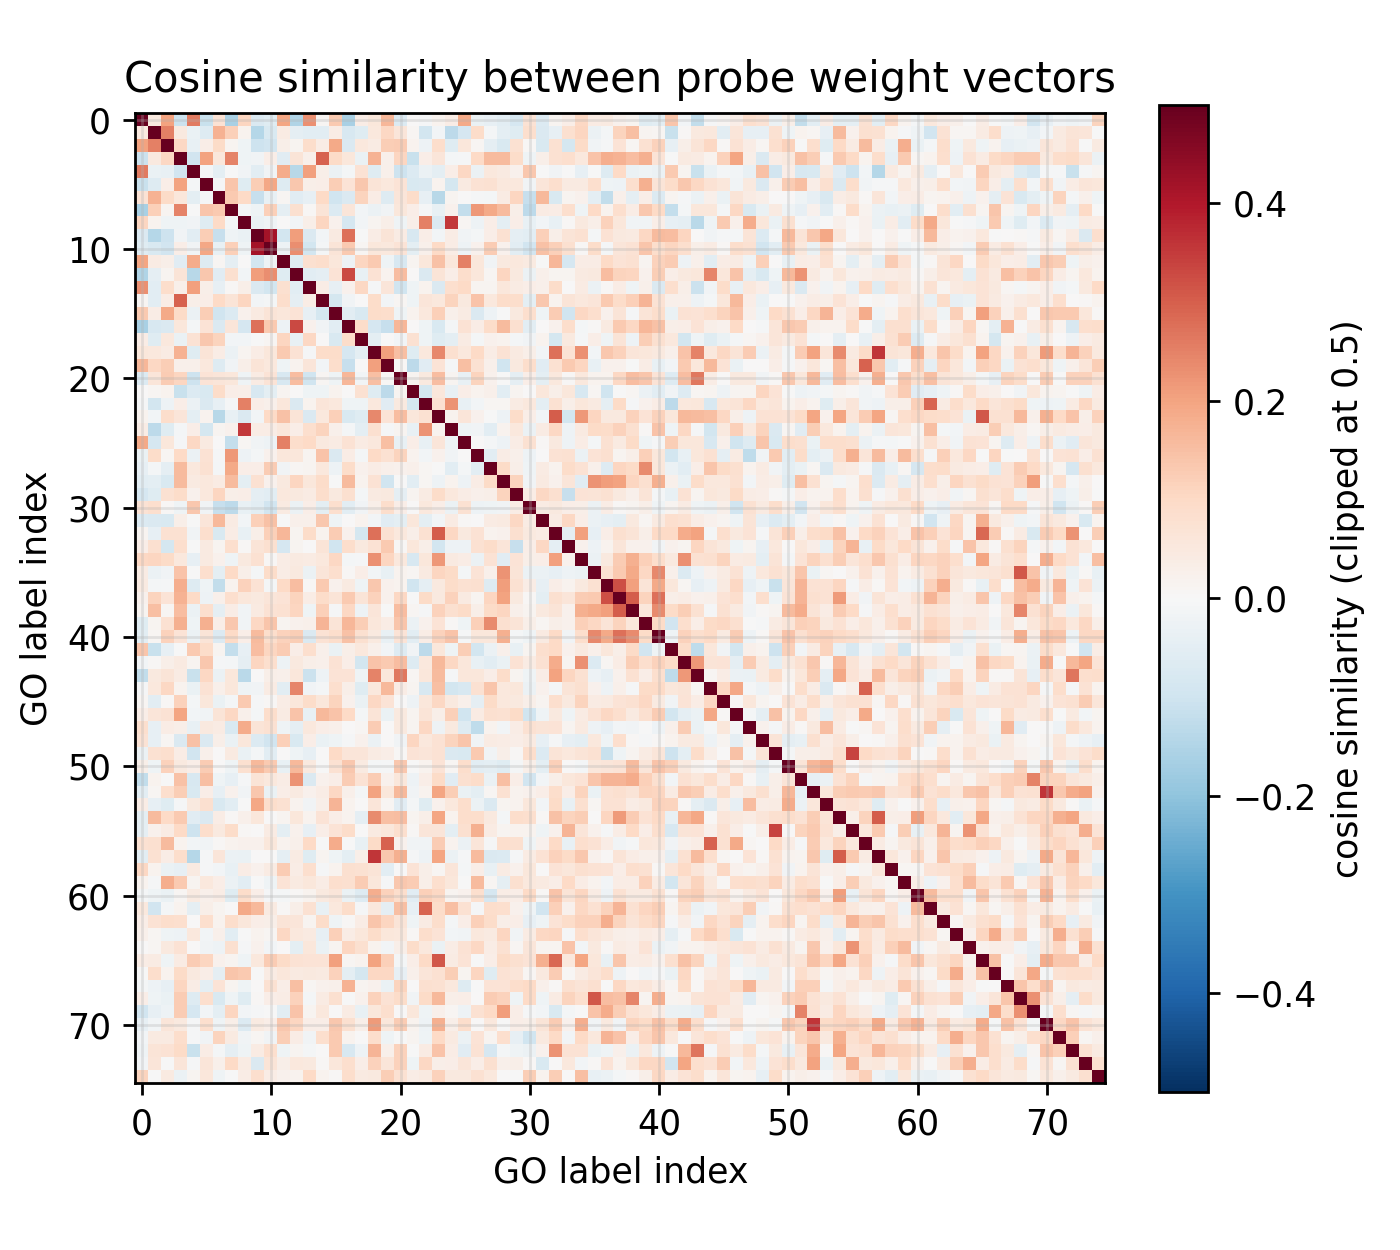
\includegraphics[width=0.62\textwidth]{fig_cosine_matrix.png}
\caption{Cosine similarity between the 75 probe weight vectors (colour scale
clipped at $\pm 0.5$). Off-diagonal similarities are small but structured: a few
pairs and a small cluster of endoplasmic-reticulum terms reach 0.2-0.4, and no pair
approaches 1.}
\label{fig:cosine}
\end{figure}

Spearman's rank correlation is $\rho = 0.5074$ (nominal
$p = 1.7 \times 10^{-181}$). After residualizing both variables on the rank of
$\log(1+q_{ij})$, the partial rank correlation is $0.4889$ (nominal
$p = 1.0 \times 10^{-166}$). The association therefore survives the co-occurrence
control and is not an artefact of frequency.

The strongest pairs are biologically adjacent: endoplasmic reticulum membrane
versus endoplasmic reticulum ($c = 0.418$, $r = 0.406$, 332 shared proteins),
presynaptic versus postsynaptic membrane, and glutamatergic synapse versus
postsynapse. The anti-aligned end pairs the nucleus with peripheral compartments
such as the extracellular exosome ($c = -0.161$, $r = -0.059$). Among the 1,218
pairs with non-positive label correlation the largest cosine is still 0.192, so the
relationship is a strong trend rather than a deterministic rule.

Taken with Section~4.3, these results describe a consistent picture: the probe
assigns similar directions to labels that co-occur, and the resulting correlation
among rows is what produces the moderately concentrated spectrum.

\section{Discussion}

\subsection{What the geometry shows}

Three statements are supported by the data. The 75 probe directions are linearly
independent with a wide margin, so there is no exact redundancy. Their spectrum is
moderately concentrated, with an effective rank of 54.54 and 49 directions needed
for 90\% of the energy. And the concentration is reproduced when the co-occurrence
structure of the labels is preserved but its association with the proteins is
destroyed.

The third statement is the informative one. It says that the geometry of $W$ is a
read-out of the label distribution: terms such as ``endoplasmic reticulum'' and
``endoplasmic reticulum membrane'' are almost always co-annotated, so their probes
converge on similar directions, and the set of 75 directions is more correlated
than random. No property of ESM-2 is needed to explain the spectrum beyond the
fact that it supports a linear read-out at all.

\subsection{Why this is not evidence of superposition}

The superposition hypothesis \cite{elhage2022toy} is about capacity: a network
encodes more features than it has dimensions and accepts interference as the
price. Nothing analogous applies here. The probe maps 480-dimensional embeddings to
75 labels, so its 75 directions live in a space more than six times larger than the
number of features; there is no pressure to share them. The regime here is the
opposite of capacity pressure: the probe has far more dimensions available than
labels to represent.

This is also why the observed effective rank of 54.54 is expected rather than
surprising. Correlated labels produce correlated rows, and correlated rows produce
a spectrum that falls short of full rank. The number 54.54 is a statement about how
redundant the GO CC annotation is, not about how the model stores features.

Establishing superposition would require different evidence: features that
outnumber dimensions, interference that can be measured behaviourally, causal
interventions on individual directions, or sparse dictionary recovery that
recovers more features than the representation dimension. None of these is
available from a set of independent logistic probes.

\subsection{Limitations}

\begin{enumerate}[leftmargin=*]
    \item \textbf{Data scope.} The download is capped at 10{,}000 reviewed
    records, and only 75 GO CC terms pass the 100-protein threshold. The dataset is
    a prefix of reviewed Swiss-Prot, so the absolute numbers are not comparable
    across papers.

    \item \textbf{Single split, no homology control.} A single 80/20 split is used,
    without homology-aware partitioning. Proteins with near-identical sequences can
    appear in both halves, which would inflate the ROC-AUC. The geometry analysis
    does not depend on the test split, but the reported performance does.

    \item \textbf{One representation.} Only layer 12 of \texttt{esm2\_t12\_35M} is
    probed, with mean pooling. Other layers, pooling schemes, regularisation
    strengths, and larger checkpoints may produce different spectra.

    \item \textbf{Dependent label pairs.} The 2{,}775 pairs share labels, so the
    nominal $p$-values of Section~4.4 are descriptive rather than inferential.
    Label-level or protein-level resampling would be required for formal inference.

    \item \textbf{Null-model scope.} Each null preserves a different subset of the
    problem, and none preserves everything. The row-permutation null destroys the
    protein-label pairing entirely, so it describes what labels alone can produce;
    it does not prove that labels are the only cause of the observed spectrum.

    \item \textbf{Ontology structure.} GO terms are related by \texttt{is\_a} and
    \texttt{part\_of}, and no propagation over the ontology is applied. Part of the
    co-occurrence structure is therefore ontological rather than empirical.
\end{enumerate}

\subsection{Future work}

\begin{enumerate}[leftmargin=*]
    \item \textbf{Capacity-constrained probes.} Represent the same labels in a
    space smaller than 75 dimensions, so that directions must be shared, and check
    whether prediction degrades in the pattern superposition predicts. This is the
    test that most directly addresses the hypothesis.

    \item \textbf{Stability of the leading subspace.} Refit $W$ on repeated
    training subsets, regularisation strengths, and random seeds, and compare the
    leading $k$-dimensional subspaces. For orthonormal bases $Q_1, Q_2$ of two
    subspaces, the similarity
    \begin{equation}
        S = \frac{\lVert Q_1^\top Q_2 \rVert_F^2}{k}
    \end{equation}
    lies in $[0,1]$. A subspace that is stable across seeds reflects the task; one
    that moves reflects optimisation.

    \item \textbf{Layers and pooling.} Repeat the analysis for other ESM-2 layers,
    attention-weighted pooling, and larger checkpoints. If the concentration is
    inherited from the labels, it should be largely invariant to these choices.

    \item \textbf{Homology-aware evaluation.} Partition train and test by sequence
    similarity rather than at random, and report per-label metrics with confidence
    intervals from repeated splits.

    \item \textbf{Ontology-aware labels.} Propagate annotations over the GO
    graph, which would make the dependence between labels explicit and test
    whether the residual concentration survives once ontology structure is
    modelled directly.
\end{enumerate}

\section{Reproducibility}

All results are produced by two notebooks:

\begin{itemize}[leftmargin=*]
    \item \texttt{Protein.ipynb} builds the dataset: it downloads the UniProt
    records, filters and parses the GO annotations, selects the labels, and computes
    the ESM-2 embeddings.
    \item \texttt{protein\_go\_geometry.ipynb} contains every analysis reported
    here: the probe, the rank checks, the spectrum, the three null-model families,
    the label-structure analysis, and the figures. It starts from the cached arrays in
    \texttt{protein\_dataset/} and runs in about 11 minutes on a CPU, dominated by
    the 300 probe refits of the permutation nulls.
\end{itemize}

The analysis notebook writes \texttt{results.json}, which holds the main statistics
quoted in this report, and the five figures in \texttt{figures/}. Re-running it regenerates
both, so the manuscript can be checked against the code by comparing
\texttt{results.json} with the tables above. The probe weight matrix is saved to
\texttt{protein\_dataset/probe\_weights.npy} so that later sections can be re-run
without refitting.

\section{Conclusion}

For 75 GO Cellular Component labels represented in 480-dimensional ESM-2
embeddings, the probe weight matrix is linearly independent, has no near-collinear
pair, and shows moderate spectral concentration (effective rank 54.54, Rank90 49).

That concentration is not evidence that the representation stores features in
shared directions. A null model that preserves the co-occurrence structure of the
labels but breaks its association with the proteins reproduces the observed
spectrum almost exactly (54.32, $p = 0.73$), while nulls that destroy the label
structure do not. The geometry of the probe is a read-out of how redundant the GO
annotations are, and with 75 labels in 480 dimensions there is no capacity pressure
that would make superposition necessary.

Weight-vector similarity nevertheless tracks label co-annotation (Spearman 0.5074,
partial 0.4889), so the probe's directions remain semantically interpretable at the
level of pairs. The distinction matters: the directions are meaningful, but their
global geometry is inherited rather than learned.

\section*{Author contributions}

R.M. designed the analysis, implemented the code, and wrote the manuscript. G.L.
contributed to the project.

\begin{thebibliography}{9}

\bibitem{elhage2022toy}
N. Elhage, T. Hume, C. Olsson, N. Schiefer, T. Henighan, S. Kravec,
Z. Hatfield-Dodds, R. Lasenby, D. Drain, C. Chen, R. Grosse, S. McCandlish,
J. Kaplan, D. Amodei, M. Wattenberg, and C. Olah.
\newblock \emph{Toy Models of Superposition}.
\newblock arXiv:2209.10652, 2022.
\newblock \url{https://arxiv.org/abs/2209.10652}.

\bibitem{lin2023esm}
Z. Lin, H. Akin, R. Rao, B. Hie, Z. Zhu, W. Lu, A. dos Santos Costa,
M. Fazel-Zarandi, T. Sercu, and A. Rives.
\newblock Evolutionary-scale prediction of atomic-level protein structure with a
language model.
\newblock \emph{Science}, 379(6637):1123--1130, 2023.
\newblock \url{https://doi.org/10.1126/science.ade2574}.

\bibitem{uniprotEmbeddings}
UniProt Consortium.
\newblock \emph{Embeddings}.
\newblock UniProt Help documentation.
\newblock \url{https://www.uniprot.org/help/embeddings}.

\bibitem{geneontology2021}
The Gene Ontology Consortium.
\newblock The Gene Ontology resource: enriching a GOld mine.
\newblock \emph{Nucleic Acids Research}, 49(D1):D325--D334, 2021.
\newblock \url{https://doi.org/10.1093/nar/gkaa1113}.

\end{thebibliography}

\end{document}
